\section{What TDE's ten points bought}\label{sec:sggaudit}

\begin{figure*}[t]
\centering
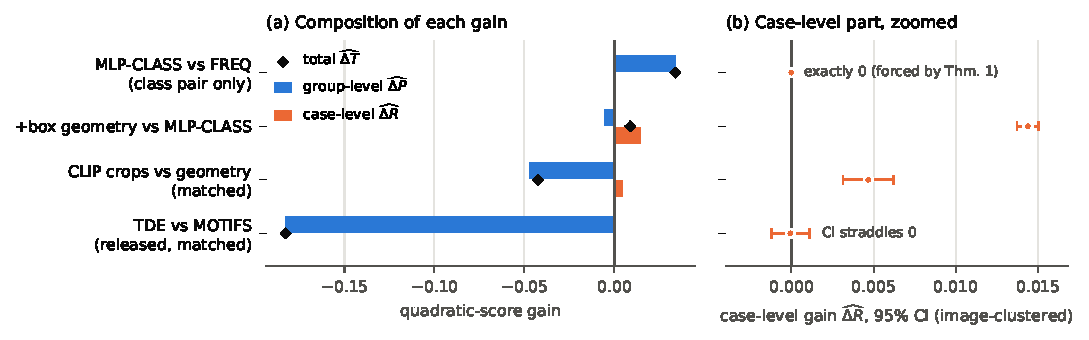
\includegraphics[width=\textwidth]{figures/fig2_where_gains_live.pdf}
\caption{\textbf{Where each gain in this paper lives}, under the quadratic score. (a) Every
comparison's total gain $\hdT$ (diamond) split into its group-level part $\hdP$ and
case-level part $\hdR$; the two parts sum to the total exactly. (b) The case-level part
alone with its image-clustered 95\% interval. Two models built from the class pair alone
differ by a purely group-level gain, as \cref{thm:population} forces. Box geometry and CLIP
crops each buy a significant case-level gain, the CLIP model despite losing on the total.
TDE's large proper-score change is group-level, with a case-level part whose interval
straddles zero.}
\label{fig:where}
\end{figure*}

Tang \etal~\cite{tang2020unbiased} release a causal MOTIFS PredCls checkpoint that yields two
models from one set of weights: the baseline (MOTIFS-SUM) and its Total Direct Effect
counterpart (MOTIFS-TDE), which subtracts a context-only counterfactual prediction at
inference. We evaluate both with the authors' own code on the canonical VG150 test split, so
the two prediction sets are aligned relation for relation. The reproduction matches the
published behaviour: the baseline reaches $R@50=0.6612$ with $mR@50=0.1459$, and TDE trades
the former for the latter, reaching $mR@50=0.2476$ and raising zero-shot recall to
$zR@50=0.1432$, while top-1 predicate accuracy falls from $0.6981$ to $0.5577$. The audit
covers $183{,}639$ relations over $26{,}446$ images in $7{,}127$ subject--object cells;
$98.9\%$ of the relations fall in the $5{,}044$ cells holding at least two, and so are
identified.

\begin{table}[t]
\centering
\footnotesize
\setlength\tabcolsep{2.6pt}
\caption{\textbf{TDE against its MOTIFS baseline} on VG150 PredCls, released checkpoints.
Raw rows use every identified relation; matched rows fit each model's temperature on a
held-out half of the images and audit the other half. The interval on $\hdR$ is
image-clustered. Our reading is the matched quadratic row; all five are reported because the
answer depends on the configuration.}
\label{tab:sggaudit}
\begin{tabular}{@{}lllrrr@{}}
\toprule
& Score & $\phi$ & $\hdT$ & $\hdP$ & $\hdR$ [95\% CI] \\
\midrule
raw & quad. & pair & $-0.11651$ & $-0.10296$ & $-0.01355$ \\
& & & & & {\scriptsize$[-0.01504,-0.01206]$} \\
raw & log & pair & $+0.03277$ & $+0.15897$ & $-0.12619$ \\
& & & & & {\scriptsize$[-0.13093,-0.12145]$} \\
raw & quad. & subject & $-0.11536$ & $+0.10175$ & $-0.21711$ \\
\midrule
matched & quad. & pair & $-0.18264$ & $-0.18258$ & $-0.00006$ \\
& & & & & {\scriptsize$[-0.00120,+0.00109]$} \\
matched & log & pair & $-0.54760$ & $-0.59157$ & $+0.04396$ \\
& & & & & {\scriptsize$[+0.04079,+0.04714]$} \\
\bottomrule
\end{tabular}
\end{table}

\paragraph{The released pair must be confidence-matched.} The two models differ sharply in
calibration: the temperatures fitted on held-out images are $T^*=2.50$ for the baseline and
$0.92$ for TDE. Scored as they ship, they give a significant case-level \emph{loss} for TDE
($-0.01355$, \cref{tab:sggaudit}), but \cref{sec:simulation} showed that a calibration
difference alone manufactures exactly that kind of loss. We therefore read the matched rows.

\paragraph{Result.} Once each model carries its own held-out temperature, TDE's
quadratic-score change is $-0.18264$, of which $-0.18258$ is group-level. The case-level part
is $\hdR=-0.00006$, interval $[-0.00120,+0.00109]$, randomization $p=.555$: indistinguishable
from zero (\cref{fig:where}). Under the log score the case-level part is small and positive, $+0.04396$ with an
interval excluding zero, against a group-level change of $-0.59157$. The two proper scores
thus disagree on whether any case-level change survives matching, and agree that whichever
is right it is at most a twelfth the size of the total. Both are well-posed: each Bregman
score defines its own exact estimand (\cref{thm:bregman}), so choosing between them is a
declaration and not an error to argue away. What both support is that TDE's change to the
predictive distribution is overwhelmingly group-level.

\paragraph{What that does and does not license.} Mean recall rose ten points; the matched
case-level gain is $-0.00006$. Those are different units and we supply no bridge between
them: it would be wrong to say ten points bought $0.00006$ of evidence, and equally wrong to
say the mean-recall gain \emph{is} group-level, since the group-level part of the proper score
fell. What the audit supports is a conjunction. The headline metric moved ten points, and
the proper-score difference behind it lives almost entirely in how the model distributes
probability across predicates within each object pair. A reader may conclude that the
ten points are not evidence of better recognition of individual relations. This
characterises TDE rather than indicting it: subtracting a context-only prediction is a
group-level intervention by construction, and the split confirms that it acts as designed.
What it questions is the habit of reading a mean-recall gain as better recognition.

\paragraph{The answer depends on the configuration.} The five rows give case-level gains of
$-0.21711$, $-0.12619$, $-0.01355$, $-0.00006$ and $+0.04396$. At two of the five,
``overwhelmingly group-level'' is false: the raw log row has $|\hdR|=0.126$ against
$|\hdP|=0.159$, and the subject-only row has $-0.217$ dominating $+0.102$. We argue for the
matched class-pair row on stated grounds --- a proper score punishes miscalibration, so
calibration must be held fixed; and coarsening is not neutral (\cref{prop:coarsen}), so the
finest grouping the benchmark defends is the conservative one --- and report the rest so that
a reader who rejects those grounds can see what follows instead.
